\chapter{Programming Interface for {\MPI} and {\OMP}}

   This chapter describes the programming interface for {\MPI} and {\OMP},
   which are widely used for parallel programming for cluster computing.
   Users can introduce {\MPI} and {\OMP} functions to {\XMP} using the interface.   

\section{{\MPI} Interface}

   {\XMP} provides the following user API functions to mix {\MPI}
   functions with {\XMP}.

\begin{itemize}
\item {\tt xmp\_get\_mpi\_comm}
\item {\tt xmp\_init\_mpi}
\item {\tt xmp\_finalize\_mpi}
\end{itemize}

\subsection{\tt xmp\_get\_mpi\_comm}
\index{xmp\_get\_mpi\_comm@{\tt xmp\_get\_mpi\_comm}}

\subsubsection*{Format}

\begin{tabular}{lll}
\verb![F]!&  {\tt integer function}& {\tt xmp\_get\_mpi\_comm()}\\
\verb![C]!&  {\tt MPI\_Comm}& {\tt xmp\_get\_mpi\_comm(void)}
\end{tabular}

\subsubsection*{Synopsis}

   {\tt xmp\_get\_mpi\_comm} returns the handle of the communicator
   associated with the executing node set. 

\subsubsection*{Arguments}

none.

\subsection{\tt xmp\_init\_mpi}
\index{xmp\_init\_mpi@{\tt xmp\_init\_mpi}}

\subsubsection*{Format}

\begin{tabular}{lll}
\verb![F]!&  {\tt }& {\tt xmp\_init\_mpi()}\\

\verb![C]!&  {\tt void}& {\tt xmp\_init\_mpi(int *args, char ***argv)}
\end{tabular}

\subsubsection*{Synopsis}

   {\tt xmp\_init\_mpi} initializes the MPI execution environment.

\subsubsection*{Arguments}

   In {\XMPC}, the command-line arguments {\tt argc} and {\tt argv}
   should be given to {\tt xmp\_init\_mpi}.


\subsection{\tt xmp\_finalzie\_mpi}
\index{xmp\_finalzie\_mpi@{\tt xmp\_finalzie\_mpi}}

\subsubsection*{Format}

\begin{tabular}{lll}
\verb![F]!&  {\tt }& {\tt xmp\_finalize\_mpi()}\\

\verb![C]!&  {\tt void}& {\tt xmp\_finalize\_mpi(void)}
\end{tabular}

\subsubsection*{Synopsis}

   {\tt xmp\_finalize\_mpi} terminates the MPI execution enviroment.

\subsubsection*{Arguments}

   none.

\subsection*{Example}
\index{Example!MPI interface}

\begin{XCexample}
#include <stdio.h>
#include "mpi.h"
#include "xmp.h"

#pragma xmp nodes p(4)

int main(int argc, char *argv[]) {
  xmp_init_mpi(&argc, &argv)

  int rank, size;
  MPI_Comm_rank(MPI_COMM_WORLD, &rank);
  MPI_Comm_size(MPI_COMM_WORLD, &size);

#pragma xmp task on p(2:3)
{
  MPI_Comm comm = xmp_get_mpi_comm(); // get the MPI communicator of p(2:3)

  int rank, size;
  MPI_Comm_rank(comm, &rank);
  MPI_Comm_size(comm, &size);
}

  xmp_finalize_mpi();

  return 0;
}
\end{XCexample}


\section{{\OMP}}
\index{Directive!threads clause@{\tt threads} clause}
\index{threads clause@{\tt threads} clause}

   Thread-level parallelism is needed to program multi-core cluster system.
   Users can use some {\OMP} features to parallelize loops in
   thread level with the {\tt threads} clause of the {\tt loop}
   directive. No direct use of {\OMP} directives in {\XMP} code is
   allowed.

\subsection*{Syntax}
\Syntax{loop}

\begin{tabular}{ll}
\verb![F]! & \verb|!$xmp| {\tt loop} {\openb} \verb|(| {\it loop-index}
 {\openb}, {\it loop-index}{\closeb}... \verb|)| {\closeb} \\
 & \hspace{3cm}{\tt on} \{{\it nodes-ref} $\vert$ {\it template-ref}\}
     {\openb} {\it reduction-clause} {\closeb}...
     {\openb} {\it threads-clause} {\closeb} \\
 & {\it do-loops} \\
 & \\
\verb![C]! & \verb|#pragma xmp| {\tt loop} {\openb} \verb|(| {\it
     loop-index} {\openb}, {\it loop-index}{\closeb}... \verb|)|
     {\closeb} \\
 & \hspace{3cm}{\tt on} \{{\it nodes-ref} $\vert$ {\it template-ref}\}
     {\openb} {\it reduction-clause} {\closeb}...
     {\openb} {\it threads-clause} {\closeb} \\
 & {\it for-loops} \\
\end{tabular}

\vspace{0.3cm}

where {\it threads-clause} is:

\vspace{0.3cm}

\begin{tabular}{ll}
 & {\tt threads} {\openb} {\it omp-clause} {\closeb} \\
\end{tabular}

\vspace{0.3cm}

and {\it omp-clause} is one of:

\vspace{0.3cm}

\begin{tabular}{ll}
 & {\tt num\_threads(} {\it num-thread} {\tt )}\\
 & {\tt private(} {\it list} {\tt )}\\
 & {\tt firstprivate(} {\it list} {\tt )}\\
 & {\tt lastprivate(} {\it list} {\tt )}\\
\end{tabular}

\subsection*{Description}

   {\OMP} clauses such as {\tt num\_threads} can be specified in {\tt
   threads} clause.
   The {\XMP} compiler generates internally {\OMP} directives from the
   {\tt loop} directive and the {\tt threads} clause.
   Note that no {\tt reduction} need to be specified in the {\tt
   threads} clause because it is inherited from the {\tt reduction}
   clause in the {\tt loop} directive.

\subsection*{Example}
\index{Example!OpenMP interface}

   This example calculates the total sum of an array.
   A {\tt threads} clause is given to the {\tt loop} directive to
   parallelize the loop statement in both process and
   thread level. 
   The {\tt reduction} clause in the {\tt loop} directive is also
   applied to the {\OMP} directive which is generated by the {\XMP}
   compiler.

\begin{XCexample}
#include <stdio.h>
#include "xmp.h"
#define N 1024

#pragma xmp nodes p(*)
#pragma xmp template t(0:N-1)
#pragma xmp distribute t(block) onto p
#pragma xmp align a[i] with t(i)

int main(void) {
  . . . // initialize a[]

  int sum = 0;
#pragma xmp loop on t(i) reduction(+:sum) threads num_threads(4)
  for (int i = 0; i < N; i++) {
    sum += a[i];
  }

  return 0;
}
\end{XCexample}


\chapter{Interface to Numerical Libraries}
\label{chap:Interface to Numerical Libraries}

   This chapter describes the XcalableMP interfaces to existing MPI
   parallel libraries, which is effective to achieve high productivity
   and performance ot {\XMP} programs.
   
\section{General rule}

   This section shows a way how existing numerical library routines are used in
   {\XMP} programs.


\begin{itemize}
\item Execution flow of XcalableMP program using XcalableMP interface is the following:\\
      XMP directive decraration $\to$ XMP interface ($\to$ native numerical library routines)
\item The name of XcalableMP interface prefixes "{\tt XMP\_}" or "{\tt xmp\_}" 
      to numerical library routine name.
\item In case that native numerical library routine needs descriptor information,
      XcalableMP interface to that numericalI library routine have an argument of 
      {\tt xmp\_desc\_t} type. A {\XMP} interface is implemented using some 
      query subroutines provided by {\XMP}.
\item A design of XMP interface to existing numerical library do not affect 
      original communication process of that numerical library.
\end{itemize}

\begin{myfigure}
 \rotatebox{-90}{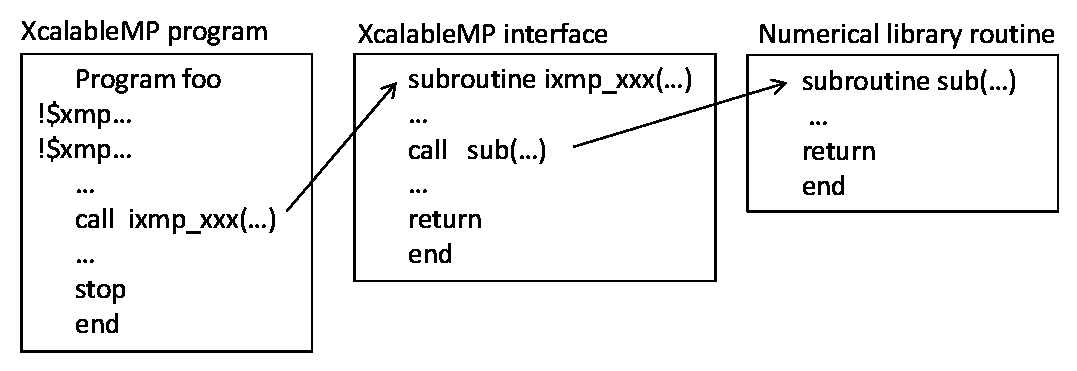
\includegraphics[scale=0.6]{figs/figb.1.eps}}
 \caption{Execution flow of XcalableMP program using XcalableMP interface}
 \label{figb.1}
\end{myfigure}

Examples of query subroutine specifications are the following.

\subsection{\tt xmp\_ga\_size}

\subsubsection*{Format}

\begin{tabular}{lll}

\verb![F]!& {\tt subroutine}& {\tt xmp\_ga\_size(d, size)}\\
          & {\tt xmp\_desc\_t} & {\tt d}\\
          & {\tt integer} & {\tt size(dim)}\\

\verb![C]!&  {\tt void}& {\tt xmp\_ga\_size(xmp\_desc\_t* d, int size[])}\\

\end{tabular}

\subsubsection*{Synopsis}

The {\tt xmp\_ga\_size} routine returns the length of each dimension of the global array.

\subsubsection*{Arguments}

\begin{itemize}
 \item {\tt d} is a descriptor, that is, an object of type {\tt
       xmp\_desc\_t} that is associated with the target global array.
 \item {\tt size} is one-dimensional integer array. {\tt dim} is the dimension 
       of the global array.
\end{itemize}

\subsection{\tt xmp\_la\_size}

\subsubsection*{Format}

\begin{tabular}{lll}

\verb![F]!& {\tt subroutine}& {\tt xmp\_la\_size(d, size)}\\
          & {\tt xmp\_desc\_t} & {\tt d}\\
          & {\tt integer} & {\tt size(dim)}\\

\verb![C]!&  {\tt void}& {\tt xmp\_la\_size(xmp\_desc\_t* d, int size[])}\\

\end{tabular}

\subsubsection*{Synopsis}

The {\tt xmp\_la\_size} routine returns the length of each dimension of
 the distributed local array.

\subsubsection*{Arguments}

\begin{itemize}
 \item {\tt d} is a descriptor, that is, an object of type {\tt
       xmp\_desc\_t} that is associated with the target global array.
 \item {\tt size} is one-dimensional integer array. {\tt dim} is the dimension 
       of the distributed local array.
\end{itemize}

\subsection{\tt xmp\_ga\_template\_unitsize}

\subsubsection*{Format}

\begin{tabular}{lll}

\verb![F]!&  {\tt subroutine}& {\tt xmp\_ga\_template\_unitsize(d, unitsize)}\\
          & {\tt xmp\_desc\_t} & {\tt d}\\
          & {\tt integer} & {\tt unitsize(dim)}\\

\verb![C]!&  {\tt void}& {\tt xmp\_ga\_template\_unitsize(xmp\_desc\_t* d, int unitsize[])}\\

\end{tabular}

\subsubsection*{Synopsis}

The {\tt xmp\_ga\_template\_unitsize} routine returns the length of each dimension of 
the template blocking factor.

\subsubsection*{Arguments}

\begin{itemize}
 \item {\tt d} is a descriptor, that is, an object of type {\tt
       xmp\_desc\_t} that is associated with the target global array.
 \item {\tt unitsize} is one-dimensional integer array. {\tt dim} is the dimension 
 of the template blocking factor associated with the target global array.
\end{itemize}


\subsection{\tt xmp\_ga\_first\_idx\_nodes\_rank}

\subsubsection*{Format}

\begin{tabular}{lll}

\verb![F]!&  {\tt subroutine}& {\tt xmp\_ga\_first\_idx\_nodes\_rank(d, rank)}\\
          & {\tt xmp\_desc\_t} & {\tt d}\\
          & {\tt integer} & {\tt rank(dim)}\\

\verb![C]!&  {\tt void}& {\tt xmp\_ga\_first\_idx\_nodes\_rank(xmp\_desc\_t* d, int rank[])}\\

\end{tabular}

\subsubsection*{Synopsis}

The {\tt xmp\_ga\_first\_idx\_nodes\_rank} routine returns node index over which 
the first row and column of global array a is distributed.

\subsubsection*{Arguments}

\begin{itemize}
 \item {\tt d} is a descriptor, that is, an object of type {\tt
       xmp\_desc\_t} that is associated with the target global array.
 \item {\tt rank} is one-dimensional integer array. {\tt dim} is the dimension of 
 node array associeted with the target global array.
\end{itemize}

\subsection{\tt xmp\_la\_lead\_dim}

\subsubsection*{Format}

\begin{tabular}{lll}

\verb![F]!&  {\tt subroutine}& {\tt xmp\_la\_lead\_dim(d, lead\_dim)}\\
          & {\tt xmp\_desc\_t} & {\tt d}\\
          & {\tt integer} & {\tt lead\_dim}\\

\verb![C]!&  {\tt void}& {\tt xmp\_la\_lead\_dim(xmp\_desc\_t* d, int lead\_dim)}\\

\end{tabular}

\subsubsection*{Synopsis}

The {\tt xmp\_la\_lead\_dim} routine returns leading dimension of local array.

\subsubsection*{Arguments}

\begin{itemize}
 \item {\tt d} is a descriptor, that is, an object of type {\tt
       xmp\_desc\_t} that is associated with the target global array.
 \item {\tt lead\_dim} is integer value.
\end{itemize}


\subsection{\tt xmp\_la\_addr}

\subsubsection*{Format}

\begin{tabular}{lll}

\verb![F]!&  {\tt subroutine}& {\tt xmp\_la\_addr(d, addr)}\\
          & {\tt xmp\_desc\_t} & {\tt d}\\
          & {\tt integer,allocatable} & {\tt addr}\\

\verb![C]!&  {\tt void}& {\tt xmp\_la\_addr(xmp\_desc\_t* d, int* addr)}\\

\end{tabular}

\subsubsection*{Synopsis}

The {\tt xmp\_la\_addr} routine returns top address of distributed local array.

\subsubsection*{Arguments}

\begin{itemize}
 \item {\tt d} is a descriptor, that is, an object of type {\tt
       xmp\_desc\_t} that is associated with the target global array.
 \item {\tt addr} is address of the start of the local array.
\end{itemize}

\section{ScaLAPACK}

   ScaLAPACK is a linear algebra library for distributed-memory.
   Communication processes of ScaLAPACK routines depend on BLACS
   (Basic Linear Algebraic Communication Subprograms).
   ScaLAPACK library routines processes in XcalableMP program also depend on 
   BLACS. This section shows a way how ScaLAPACK library routines are used in
   {\XMP} programs.

\begin{itemize}
\item For ScaLAPACK library routine having descriptor array as argument,
      the XcalableMP interface routine have BLACS context handle including 
      the descriptor array as new argument.
\item The blacs\_exit routine is unnecessary, because XcalableMP program executes process 
      corresponding to MPI\_Finalize routines.
\item A valid value of the argument "order" of BLACS routine "{\tt blacs\_gridinit}" is 
      only column-major. 
\end{itemize}

\subsection*{Example}
\begin{description}

\item[Example 1]
   This example shows implementation of {\XMPF} interface for ScaLAPACK driver routine "pdgesv".

\begin{XFexample}
      subroutine xmp_pdgesv(n,nrhs,a,ia,ja,xmp_desc_of(a),ipiv,
     *                b,ib,jb,xmp_desc_of(b),ictxt,info)
      integer n,nrhs,ia,ja,ib,jb,ictxt(2),info
      double precision a,b
      xmp_desc_t xmp_desc_of(a),xmp_desc_of(b)
      integer size_a(2),unitsize_a(2),rank_a(2),lead_dim_a,desca(9)
      integer size_b(2),unitsize_b(2),rank_b(2),lead_dim_b,descb(9)
      
      call xmp_ga_size(xmp_desc_of(a),size_a)
      call xmp_ga_template_unitsize(xmp_desc_of(a),unitsize_a)
      call xmp_ga_first_idx_nodes_rank(xmp_desc_of(a),rank_a)
      call xmp_la_lead_dim(xmp_desc_of(a),lead_dim_a)
      
      call xmp_ga_size(xmp_desc_of(b),size_b)
      call xmp_ga_template_unitsize(xmp_desc_of(b),unitsize_b)
      call xmp_ga_first_idx_nodes_rank(xmp_desc_of(b),rank_b)
      call xmp_la_lead_dim(xmp_desc_of(b),lead_dim_b)
      
      desca(1)=1
      desca(2)=ictxt(1)
      desca(3)=size_a(1)
      desca(4)=size_a(2)
      desca(5)=unitsize_a(1)
      desca(6)=unitsize_b(2)
      desca(7)=rank_a(1)
      desca(8)=rank_a(2)
      desca(9)=lead_dim_a
      
      descb(1)=1
      descb(2)=ictxt(2)
      descb(3)=size_b(1)
      descb(4)=size_b(2)
      descb(5)=unitsize_b(1)
      descb(6)=unitsize_b(2)
      descb(7)=rank_b(1)
      descb(8)=rank_b(2)
      descb(9)=lead_dim_b
      
      call pdgesv(n,nhrs,a,ia,ja,desca,ipiv,b,ib,jb,descb,info)
      
      return
      end

\end{XFexample}


\item[Example 2]
     This example shows a XcalableMP program using the interface of Example1. 

\Example{nodes}
\Example{template}
\Example{distribute}
\Example{align}
\Example{loop}
\begin{XFexample}
      program xmptdgesv

      double precision a(1000,1000)
      double precision b(1000)
      integer ipiv(2*1000,2)
!$xmp nodes p(2,2)
!$xmp nodes q(2)=p(1:2,1)
!$xmp template t(1000,1000)
!$xmp template t1(2*1000,2)
!$xmp template s(1000)
!$xmp distribute t(block,block) onto p
!$xmp distribute t1(block,block) onto p
!$xmp distribute s(block) onto q
!$xmp align a(i,j) with t(i,j)
!$xmp align ipiv(i,j) with t1(i,j)
!$xmp align b(i) with s(i)
      ...
      integer i,j,ict,ictxt(2),myrow,mycol
      integer m=1000,n=1000,nprow=2,npcol=2
      integer icontxt=-1,iwhat=0
      integer nrhs=1,ia=1,ja=1,ib=1,jb=1,info
      character*1 order
      ...
      order="C"
      ...
      call blacs_get(icontxt,iwhat,ict)
      call blacs_gridinit(ict,order,nprow,npcol)
      ...
      ictxt(1)=ict
      ictxt(2)=ict
      ...
!$xmp loop (i,j) on t(i,j)
      do i=1,m
         do j=1,n
            a(i,j) = ...
         end do
      end do
      ...
!$xmp loop on s(i)
      do i=1,m
         b(i)= ...
      end do
      ...
      call xmp_pdgesv(n,nrhs,a,ia,ja,xmp_desc_of(a),ipiv,
     *                b,ib,jb,xmp_desc_of(b),ictxt,info)
      ...
      call blacs_gridexit(ictxt)
      ...
      stop
      end
\end{XFexample}
\end{description}
